% Evaluation Pipeline Diagram
% Compile with: pdflatex eval_pipeline.tex
% Or include in main paper after loading tikz packages

\documentclass[tikz,border=8pt]{standalone}
\usepackage{tikz}
\usetikzlibrary{positioning, arrows.meta, shapes.geometric, calc, fit, backgrounds}

\begin{document}

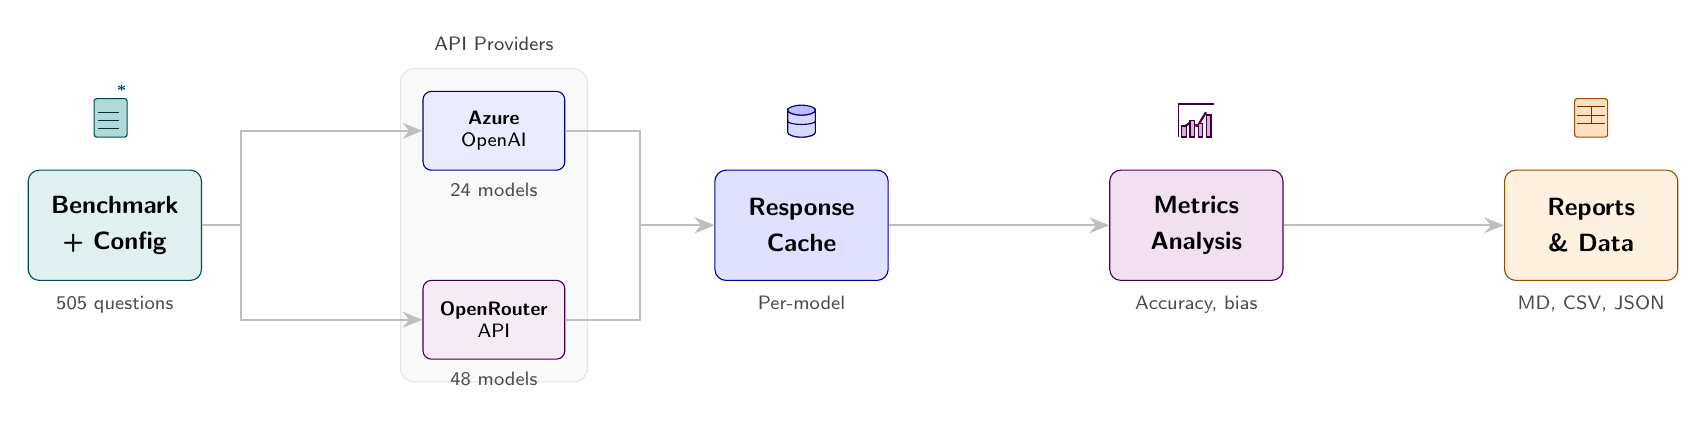
\begin{tikzpicture}[
    % Node styles
    stage/.style={
        rectangle,
        rounded corners=4pt,
        draw=#1!60!black,
        fill=#1!12,
        minimum width=2.2cm,
        minimum height=1.4cm,
        align=center,
        font=\small\sffamily
    },
    stage/.default=blue,
    provider/.style={
        rectangle,
        rounded corners=3pt,
        draw=#1!50!black,
        fill=#1!8,
        minimum width=1.8cm,
        minimum height=1cm,
        align=center,
        font=\scriptsize\sffamily
    },
    provider/.default=gray,
    arrow/.style={
        -{Stealth[length=2.5mm, width=2mm]},
        line width=0.8pt,
        draw=gray!50
    },
    sublabel/.style={
        font=\scriptsize\sffamily,
        text=gray!60!black
    }
]

% Define positions
\def\xsep{2.8cm}
\def\ysep{1.2cm}

% Stage 1: Input (Config + Benchmark)
\node[stage=teal] (input) {
    \textbf{Benchmark}\\[2pt]
    \textbf{+ Config}
};
\node[sublabel, below=2pt of input] {505 questions};

% Stage 2: API Providers (split into two)
\node[provider=blue, right=\xsep of input, yshift=\ysep] (azure) {
    \textbf{Azure}\\OpenAI
};
\node[sublabel, below=1pt of azure] {24 models};

\node[provider=violet, right=\xsep of input, yshift=-\ysep] (openrouter) {
    \textbf{OpenRouter}\\API
};
\node[sublabel, below=1pt of openrouter] {48 models};

% Provider group label - positioned above the group box
\node[font=\scriptsize\sffamily, text=gray!50!black] at ($(azure.north) + (0, 0.6)$) {API Providers};

% Stage 3: Cache
\node[stage, right=\xsep of $(azure)!0.5!(openrouter)$] (cache) {
    \textbf{Response}\\[2pt]
    \textbf{Cache}
};
\node[sublabel, below=2pt of cache] {Per-model};

% Stage 4: Analysis
\node[stage=violet, right=\xsep of cache] (analysis) {
    \textbf{Metrics}\\[2pt]
    \textbf{Analysis}
};
\node[sublabel, below=2pt of analysis] {Accuracy, bias};

% Stage 5: Output
\node[stage=orange, right=\xsep of analysis] (output) {
    \textbf{Reports}\\[2pt]
    \textbf{\& Data}
};
\node[sublabel, below=2pt of output] {MD, CSV, JSON};

% Arrows from input to providers
\draw[arrow] (input.east) -- ++(0.5,0) |- (azure.west);
\draw[arrow] (input.east) -- ++(0.5,0) |- (openrouter.west);

% Arrows from providers to cache
\draw[arrow] (azure.east) -| ($(azure.east)!0.5!(cache.west)$) |- (cache.west);
\draw[arrow] (openrouter.east) -| ($(openrouter.east)!0.5!(cache.west)$) |- (cache.west);

% Arrows to rest
\draw[arrow] (cache) -- (analysis);
\draw[arrow] (analysis) -- (output);

% Icons
\begin{scope}[yshift=0.4cm]
    % Config icon (gear + list)
    \node[above=8pt of input] {
        \tikz[scale=0.35]{
            \draw[fill=teal!30, draw=teal!60!black, rounded corners=1pt] (0,0) rectangle (1.2,1.4);
            \foreach \y in {0.3, 0.6, 0.9} {
                \draw[teal!40!black, line width=0.4pt] (0.15,\y) -- (0.9,\y);
            }
            \node[teal!60!black] at (1.0, 1.15) {\tiny\textbf{*}};
        }
    };

    % Cache icon (database cylinder)
    \node[above=8pt of cache] {
        \tikz[scale=0.35]{
            % Bottom ellipse (hidden by body)
            \draw[fill=blue!20, draw=blue!50!black] (0.6,0.2) ellipse (0.5 and 0.18);
            % Cylinder body
            \draw[fill=blue!15, draw=blue!50!black] (0.1,0.2) -- (0.1,1.0) arc (180:360:0.5 and 0.18) -- (1.1,0.2) arc (360:180:0.5 and 0.18);
            % Top ellipse
            \draw[fill=blue!25, draw=blue!50!black] (0.6,1.0) ellipse (0.5 and 0.18);
            % Middle line
            \draw[blue!40!black] (0.1,0.6) arc (180:360:0.5 and 0.12);
        }
    };

    % Analysis icon (chart with trend)
    \node[above=8pt of analysis] {
        \tikz[scale=0.35]{
            \draw[violet!50!black, line width=0.5pt] (0,0) -- (0,1.2) -- (1.3,1.2);
            \draw[violet!60!black, line width=0.8pt] (0.1,0.3) -- (0.4,0.5) -- (0.7,0.4) -- (1.0,0.9);
            \foreach \x/\h in {0.2/0.4, 0.5/0.6, 0.8/0.5, 1.1/0.8} {
                \draw[fill=violet!30, draw=violet!50!black] (\x-0.08,0) rectangle (\x+0.08,\h);
            }
        }
    };

    % Report icon (document with table)
    \node[above=8pt of output] {
        \tikz[scale=0.35]{
            \draw[fill=orange!25, draw=orange!60!black, rounded corners=1pt] (0,0) rectangle (1.2,1.4);
            \draw[orange!40!black, line width=0.3pt] (0.1,1.1) -- (1.1,1.1);
            \draw[orange!40!black, line width=0.3pt] (0.1,0.8) -- (1.1,0.8);
            \draw[orange!40!black, line width=0.3pt] (0.1,0.5) -- (1.1,0.5);
            \draw[orange!40!black, line width=0.3pt] (0.6,0.5) -- (0.6,1.1);
        }
    };
\end{scope}

% Background for providers group
\begin{scope}[on background layer]
    \node[fit=(azure)(openrouter), inner sep=8pt, fill=gray!5, rounded corners=5pt, draw=gray!20] {};
\end{scope}


\end{tikzpicture}

\end{document}
